\documentclass[a4paper,11pt]{amsart}
\usepackage{amssymb}
\usepackage{graphicx}

\parskip 1ex
\parindent 0 pt

\newcounter{temp}
\newcounter{prob_counter}
\newcounter{sprob_counter}

\newenvironment{problem}
{\begin{list}{{\bf \arabic{prob_counter}}}{
      \usecounter{prob_counter}
      \addtolength{\labelsep}{.6ex}
      \addtolength{\itemsep}{4.3ex}
      \setlength{\leftmargin}{1.4em}}
      \setcounter{prob_counter}{\value{temp}}
}
{\setcounter{temp}{\value{prob_counter}}  
  \end{list}
}

\newenvironment{subprob}
{
  \begin{list}{{\bf \alph{sprob_counter}}}{
      \usecounter{sprob_counter}
      \addtolength{\labelsep}{.6ex}
      \addtolength{\itemsep}{.5ex}
      \setlength{\leftmargin}{1.7em}}
}
{\end{list}}

\newenvironment{solution}{\textbf{Solution.}}{\qed}

\newcommand{\rubrik}[1]{\bigskip \begin{center}{\bf #1}\end{center} \medskip}

\newcommand{\NN}{\mathbb{N}}
\newcommand{\ZZ}{\mathbb{Z}}
\newcommand{\QQ}{\mathbb{Q}}
\newcommand{\RR}{\mathbb{R}}




\begin{document}

\pagestyle{empty}
\thispagestyle{empty}

{\small{\sc\noindent
        Sebastian Plenz ({\tt sebastianp16@ru.is}) and Axel Steingrimsson ({\tt axels16@ru.is})
}}

\rubrik{PROBLEM SET 3 (T-445-GRTH)}

You need to collect $\bf 65$ points to get a full score {\bf but} you cannot get more than {\bf X} points (in total) from a problem section with annotation {\bf max X}.

{\bf Please make sure to:}\\
1. Write your name/email(s) on your work (replace my name above).\\
2. Write your answers in \texttt{{\textbackslash}begin\{solution\} ... {\textbackslash}end\{solution\}} blocks given after each problem. Turn in a single \LaTeX-generated pdf.\\
3. Write clear and concise proofs: points may be deducted for vagueness.




\section{Connectivity and Cuts ({\bf max 22})}

Below, $\mathcal{B}(G)$ denotes the set of blocks of graph $G$.

\begin{problem}
 \item (5 points) Show that for all $1 \le k \le k'$ there is a graph with $\kappa(G) = k$ and $\kappa'(G) = k'$. 
\end{problem}
\begin{solution}
	We create a graph with these values. Consider two complete graphs on $k'$ vertices. Take $k$ more vertices and connect them with $2 \cdot k'$ edges to all of the vertices of each complete graph. Additionally connect each of the vertices with each other new vertices with $k'$ edges. The resulting graph has $\kappa(G) = k$ and $\kappa'(G) = k'$. \\
	The following picture is an example for $\kappa(G) = 2$ and $\kappa'(G) = 4 $. \\
	\includegraphics{A1.jpg}
\end{solution}

\begin{problem}
  \item (5 points) For $n \ge 2$, show that for any connected $n$-vertex graph $G$, $|\mathcal{B}(G)|\le n-1$.
 Moreover, show that such a graph has exactly $n-1$ blocks if, and only if, it is a tree on $n$ vertices.
\end{problem}
\begin{solution}
	The number of blocks is maximal if there are no cycles. This means, the number of blocks is maximal for a tree. Otherwise a cycle contains more than two vertices and creates a block, so in total we have less blocks. In a tree, every two adjacent vertices create a block, therefor the number of blocks is equal to $n-1$ and this proves the claim. 
\end{solution}


\begin{problem}
\item (8 points) For a graph $G$, define its \textit{block graph} $B(G)$ as the graph with vertex set $\mathcal{B}(G)$, where two blocks $B_1$ and $B_2$ are adjacent if, and only if, $B_1 \cap B_2 \ne \varnothing$.
 Show that in the graph $B(G)$, each block is a complete subgraph.
\end{problem}
\begin{solution}
	Let $G$ be a connected graph. 
	Then let $B(G)$ be be the block graph of $G$ with the vertex set $\mathcal{B}(G)$, 
	where two blocks $B_1$ and $B_2$ are adjacent if, and only if, $B_1 \cap B_2 \ne \varnothing$.
	Then for each block in $B(G)$, $B_i$, create a vertex called $B_i$ and connect each block $B_i$ and $B_j$ by an edge if,
	 and only if, the blocks share a vertex in $G$.
	Then every block in $B(G)$ contains two vertices, one vertex representing a block in $G$, $B_I$, 
	and one vertex representing a common vertex between two adjacent blocks in $G$.
	Therefore each block in $B(G)$ contains two vertices and one edge which is equal to a $K_2$ graph.
	Therefore every block in $B(G)$ is a complete subgraph. 
\end{solution}


\begin{problem}
\item (10 points) Let $G$ be a connected graph. For each vertex $u \in V(G)$, let $b(u)$ denote the number of blocks in $G$ that contain $u$. Show that the number of blocks of $G$ is given by
 $
  |\mathcal{B}(G)| = 1 + \sum_{u \in V(G)} (b(u) - 1).
 $
\end{problem}
\begin{solution}
	Let $G$ be a connected graph. 
	Let $C(G) \subset V(G)$ be the set of cut-vertices of $G$.
	Let $B_1, ..., B_i$ be the set of blocks in $G$.
	Then every block in $G$, $B_i$ contains $u \geq 1, u \in C(G)$.
	Then we know that $G$ is a connected graph so each $u \in C(G), b(u) \geq 2$.
	And every vertex $m$ in a block $B_i$ that is not in $C(G)$ must have that $b(m) = 1$.
 	So in order to remove all the extraneous vertices from $V(G)$ sum each vertex where  $b(m) - 1 > 0$.
	Then as $G$ is a connected graph there must be at least one initial block, so 
$
  |\mathcal{B}(G)| = 1 + \sum_{u \in V(G)} (b(u) - 1).
 $
\end{solution}




\section{Flows ({\bf max 25})}


\begin{problem}
  \item (5 points) Give an example of a network with more than one maximum flow. Is it possible to have precisely two maximum
 flows? In general, is it possible to have finitely many maximum flows if the maximum flow is not unique?
\end{problem}
\begin{solution}
	An example: \\
	\includegraphics{A5.jpg} \\
	No it is not possible. If there are two different flows $f_1, f_2$ than
	$$f_s=s \cdot f_1+ (1-s) \cdot f_2; s \in (0,1) $$
	is a infinite family of maximum flows.
\end{solution}


\begin{problem}
 \item (10 points) Use the Ford-Fulkerson algorithm to find a maximum flow in the following network: 
 \begin{center} 
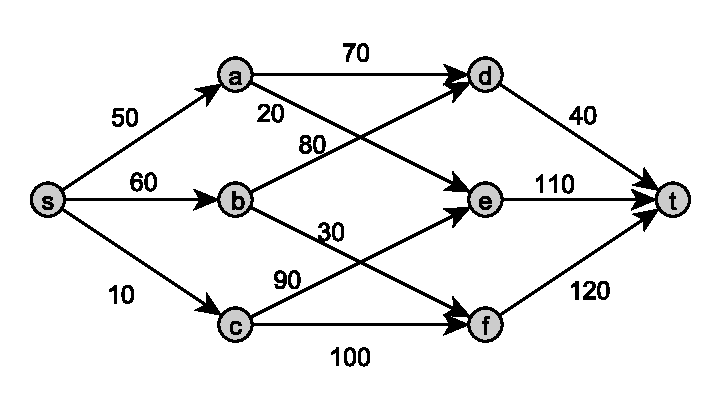
\includegraphics[height=4.5cm]{ff.pdf}  
 \end{center}
 Prove that the flow is indeed maximum by finding a source vertex cut $S$ such that $\text{val}(f) = c^+(S)$.
\end{problem}
\begin{solution}
	A possible run could look like the following pictures.\\
	\includegraphics{A6_1.jpg} \\
	\includegraphics{A6_2.jpg} \\
	\includegraphics{A6_3.jpg} \\
	\includegraphics{A6_4.jpg} \\
	\includegraphics{A6_5.jpg} \\
	This makes a maximum flow of 100. A source vertex cut to proof would be $S=\{ s, a, d, b\} $.
\end{solution}


\begin{problem}
\item (10 points) Let $\vec{G}$ be an Eulerian digraph and let $u,v \in V(\vec{G})$ be adjacent by exactly $k$ parallel directed edges with tail $u$ and head $v$. Let $\vec{G'}$ be the digraph obtained from $\vec{G}$ by removing those $k$ edges.
 Show that $\vec{G'}$ has $k$ edge-disjoint directed $v,u$-paths. 
\end{problem}
\begin{solution}
	$\vec{G}$ is a Eulerian digraph, so there exists an Eulerian Circuit on the directed graph. so, each edge with tail $u$ and head $v$ is part of a diffrent circle containing $u$. The rest of the circle is a $v,u$-path and therefor, there exists as many $v,u$-paths, as edges  with tail $u$ and head $v$ existed before removing. This has been $k$ and this shows the assumption.
\end{solution}





\section{Planar Graphs ({\bf max 45})}


\begin{problem}
\item (5 points) Consider a simple graph $G$ on six vertices $a, b, c, d, e, f$
where each pair of vertices is adjacent except for the pairs $\{a, b \}$, $\{c, d \}$, $\{e, f \}$. Is $G$ a planar graph?
\end{problem}
\begin{solution}
	The graph can be displayed as follows: \\
	\includegraphics{A8.jpg} \\
	So it is planar.
\end{solution}


\begin{problem}
 \item (10 points) Euler's formula states: Every connected plane graph with $n$ vertices, $m$ edges, and $f$ faces satisfies the  equation $n - m +f = 2$.
Prove this formula inductively by using contraction of a graph by an edge.
\end{problem}
\begin{solution}
	Start of induction: Let $n=1$. The only possible edges are cycles, that create exactly one face per edge. Additionally, we have the outside face. If $e$ denotes the number of edges, our formula says 
	$$ n-m+f=1-m+m+1=2.$$
	For an arbitrary but fixed $n\in \NN$, the assumption holds. \\
	Take a planar graph on $n+1$ vertices. We contract along an arbitrary edge, that connects two vertices. This reduces the number of vertices and the number of edges by 1. The number of faces stays the same. The equation for our graph on $n+1$ vertices is, if we consider $n_n,m_n, f_n$ to be the values of the contracted graph, 
	$$(n_n+1)-(m_n+1)+f_n=n_n-m_n+f_n=2.$$
	The last equality holds by assumption.
\end{solution}


\begin{problem}
\item  (10 points) For $n \ge 1$, consider the $n \times n$ chessboard, and let $V$ denote the $n^2$ squares of the board. Let $CH_{n} = (V, E)$ denote the simple graph on vertex set $V$ so that $\{u, v\} \in E$ if, and 
 only if, a knight at square $u$ can reach $v$ in a single move (a knight moves either two squares horizontally
 and one square vertically, or two squares vertically and one square horizontally). 
 For which values of $n$ is $CH_{n}$ planar?
\end{problem}
\begin{solution}
	For $n=1,..3$ the graph is planar. For 1 and 2, it is trivial, because these are just isolated vertices. For $n=3$, we already showed that for the solution of an other exercise. \\
	For $n \geq 4$ the graph is not planar. We only need to show it for $n=4$ because this is a subgraph of all bigger $n$ and it follows from the theorem from the lecture. $K_{3,3}$ is a minor of the graph, what can be seen by rooting the graph. By the theorem of Wagner, $CH_{4}$ and therefor $CH_{n}$ for all $n \geq 4$ is not planar.
\end{solution}


\begin{problem}
\item  Prove that: 
 \begin{subprob}
    \item (5 points) Every simple planar graph with no $3$-cycles has a vertex of degree at most $3$.
    \item (5 points) Every simple planar graph on $n \ge 4$ vertices has at least four vertices of degree at most $5$.
  \end{subprob}
\end{problem}
\begin{solution}
	a) Let $G$ be a simple planar graph with no cycle greater than 3. 
	Then let $F$ is the set of faces, $E$ is the set of edges, and $V$ is the set of vertices on $G$.
	Then we can use we can use Euler's formula where $F ? E + V = 2$.
	Then If there are no cycles greater than 3, by assumption, then each face is enclosed by at least 4 edges as a face needs at least 3 edges to be enclosed. 
	Therefore the number of faces $F$ is less than half of the number of edges: $F < E * 2$.
	Therefore the number of vertices is greater than half the edges: $V > E / 2$. 
	If all the vertices in $G$ have a degree $\geq 4$ then $ V < E / 2$
	which means that $0 < 2$ which is a contradiction. 
	So no vertex in a simple planar graph with no 3 cycles can have a degree larger than 3. \\
	b) 
\end{solution}


\begin{problem}
 \item (10 points) Show that if a simple planar graph is regular, it must be $r$-regular with $r \in \{1, 2, 3, 4, 5 \}$.
 For each $r \in \{3, 4, 5\}$, construct an infinite collection of simple planar non-isomorphic 
 $r$-regular graphs.
\end{problem}
\begin{solution}
	It can not be 6-regular or higher, because you need at least 7 vertices for that and by number 11 b) there exists vertices with maximum degree 5. Removing the five adjacent edges of this vertex creates two components, and so the maximum degree can only be 5. \\
	Take a k-complete graph. Copy this graph, remove a outer edge of each graph and connect each of the two vertices, that have been connected with the removed edges. In the following pictures, there are the 3, 4 and 5-connected graphs and a sketch of how to continue to the bigger ones. This sequences could be infinitely continued. \\
	\includegraphics{A12_1.jpg} \\
	\includegraphics{A12_2.jpg} \\
	\includegraphics{A12_3.jpg} \\
\end{solution}


\begin{problem}
\item (5 points) Show that a simple and connected $4$-regular planar graph, where each face is bounded by exactly $3$ edges,
 must have $6$ vertices, $12$ edges and $8$ faces. 
\end{problem}
\begin{solution}
	Let $n$ be the number of vertices, $m$ the number of edges and $f$ the number of faces. Every vertex has degree 4 so the number of edges is double of the number of vertices. Every edge is bounding two faces and every faces has 3 boundary edges. In equations:
	$$ m=2 \cdot n; f= \frac{2}{3}\cdot m$$
	If we use Euler's Formula, we get
	$$ \frac 1 2 \cdot m -m + \frac{2}{3}\cdot m =2 $$
	$$ \Leftrightarrow m= 12.$$
	So the claim is proofed.
\end{solution}


\begin{problem}
 \item (7 points) Let $G$ be a graph such that for every two vertices $u,v$, there are at most two vertex-disjoint paths of positive
 lengths from $u$ to $v$. Show that $G$ is planar. 
\end{problem}
\begin{solution}
\end{solution}



\section{Subdivisions ({\bf max 30})}

\begin{problem}
 \item (10 points) Show that if a graph is homeomorphic to an Eulerian graph, it is also an Eulerian graph. 
 Is a contraction of an Eulerian graph also an Eulerian graph?
 Is it true that if a graph is homeomorphic to a Hamiltonian graph, it is also Hamiltonian?
\end{problem}
\begin{solution}
	The graphs are only different by vertices of degree 2. These vertices are between two vertices $u,v$, that are part of both graphs. If there is an eulerian circuit, it uses the edge between u and v exactly once and instead of the direct vertex, it uses just the path with the vertices in between and it is still fine. \\
	Contraction does not keep eulerian graphs as you can see in the following picture. The first graph is eulerian but after contraction along the red edge, it is not eulerian anymore. \\
	\includegraphics{A15} \\
	For a Hamiltonian graph it holds because of similar reasons as for the eulerian graph.
\end{solution}


\begin{problem}
 \item (8 points) Show that for two homeomorphic graphs $G$ and $G'$,
 \[
  |V(G)| - |E(G)| = |V(G')| - |E(G')|.
 \]
\end{problem}
\begin{solution}
	The only difference between the graphs are are vertices of degree 2, that subdivide edges in more edges. Without loss of generality, $G$ has n vertices of degree 2 more than $G'$. Therefor, it has n edges more than $G'$. So
	$$  |V(G)| - |E(G)| = |V(G') + n| - |E(G')+n| $$
	$$ =|V(G)|+n -n- |E(G)| =|V(G')| - |E(G')|.$$
\end{solution}


\begin{problem}
 \item (20 points) Determine all graphs of minimal degree $3$ without two edge-disjoint cycles (recall that loops and parallel edges count as cycles).
 Using this result, prove that every $n$-vertex graph with $n+4$ edges contains two edge-disjoint cycles.
\end{problem}
\begin{solution}
	There are no vertices of degree higher than 3. If there would be a vertex with degree 4 or higher, you can seperate the adjacent edges in two parts, and because of the minimal degree for each vertex, you will find two edge-disjoint cycles. So all vertices have degree 3. It holds, that $m=\frac{3}{2} \cdot n$, and so, $n$ needs to be even. You can't have a loop, because this would lead to an other vertex with two open edges and this needs to create a cycle, because of the amount of edges per vertex you would have in the subtree(more than n-1 edges lead to a cycle on n vertices). For the case $n\geq 4$, you can not have parallel edges, with a similar proof as for the loops. For the reason in the brackets, it also needs to hold $m-c \leq n-1$ for $c$ is the length of the smallest cycle. With the formula for the edges, we know, $c \geq \frac{n}{2} +1$.
	Construction for $n\in \{2, 4, 6\}$ is possible an unique and displayed in the following graphic.\\╠
	\includegraphics{A17_1} \\
	The next one would be $n=8, c\geq 5$. If we construct a cycle of length at least 5, we would need more vertices than 8, if all the vertices have degree 3. We start with a single vertex, that has three adjacent vertices and none of them are adgacent. All of them three have two more new adjacent vertices. This makes a total number of 10 vertices and is a contradiction. \\
	\includegraphics{A17_2} \\
	With the same reason, you can not have such graphs with $n\geq 10$, so the graphs from the first graphic are all such graphs. \\
	For the second part we need to consider two diffrent cases. \\
	Case1: The length of the smallest cycle is less or equal to 4. \\
	If we remove the edges of this cycle from the graph, the graph still has at least n edges, and therefor there must still be a cycle. So, we have at least two edge-disjoint cycles. \\
	Case2: The length of the smalles cycle is greater or equal to 5. \\
	If we remove all vertices of degree 0, the graph will not loose a cycle. The same holds for vertices of degree 1, so we can remove them with their corresponding edge as well. Take a vertex $c$ of degree 2. The adjacent edges connect two vertices $u,v$. Removing those two edges and $c$ and adding the vertex $\{u,v\}$ will keep it a $n'$-vertex graph with $n'+4$ edges. $\{u,v\}$ was no edge of the graph before, because this would have created a cycle of length3. So we can remove all our vertices of degree two and keep the properties of the graph. \\
	By the first part, we know that a graph with two edge-disjoint cycles and a minimum degree of 3 does not exist for $n \geq 8$. For smaller $n$, our smallest cycle has a length less or equal than 4, and is already covered by the first case. \\
	In total, the claim is proved.	 
\end{solution}



\end{document}

